% !TEX TS-program = pdflatex

\documentclass[unicode,11pt,notheorems,xcolor=table]{beamer}
\usepackage{fix-cm}
\usepackage[T2A]{fontenc}
\usepackage[utf8]{inputenc}
\usepackage[russian]{babel}
\usepackage{amsmath,amsfonts,amssymb,amsthm}
\usepackage{mathtools}
\usepackage{diagbox}

\usepackage{ulem}
\usepackage{tikz}
\usepackage{graphicx}
%\usepackage{tkz-graph}
\usetikzlibrary{matrix,arrows,decorations.pathmorphing, arrows.meta,positioning}
\usetikzlibrary{positioning,calc}
\usetikzlibrary{patterns}
\usetikzlibrary{decorations.pathreplacing}

%Описание стиля презентации
\usetheme[sidebar=0]{kfmn} 
\setbeamercovered{transparent}

%\definecolor{cyan}{RGB}{240,217,1}
%\definecolor{vgugreen}{RGB}{143,188,103}
%\definecolor{vgured}{RGB}{234,38,40}
%\definecolor{vgublue}{RGB}{53,101,167}
\hypersetup{colorlinks,linkcolor=,urlcolor=blue}

\makeatletter
	\g@addto@macro{\endtabular}{\rowfont{}}% Clear row font
	\makeatother
	\newcommand{\rowfonttype}{}% Current row font
	\newcommand{\rowfont}[1]{% Set current row font
		\gdef\rowfonttype{#1}#1\ignorespaces%
	}
\makeatother

\newcommand{\myunit}{9mm}
\tikzset{
    node style sp/.style={draw,circle,minimum size=\myunit},
    node style ge/.style={circle,minimum size=\myunit},
    arrow style mul/.style={draw,sloped,midway,fill=white},
    arrow style plus/.style={midway,sloped,fill=white},
}

%[0, 6, 8, 8, 10, 5, 6, 10, 8, 10, 10], 

\pgfdeclareimage[height=8mm]{university-logo}{logo-iem.png}
\logo{\pgfuseimage{university-logo}}
%2[0, 11, 10, 8, 11, 5, 11, 11, 8, 11, 10, 11],

\titlepicture{
	\begin{tikzpicture}[y=1.4cm,overlay,rotate=8]
	\coordinate (O) at (-3cm,0.9cm);
	\filldraw[thick,draw= vgublue, fill=vgublue!20!white] (0,0) circle[radius=4.2cm];
	\clip (0,0) circle[radius=4.2cm];
	\draw (-1.5,1.5) node{
	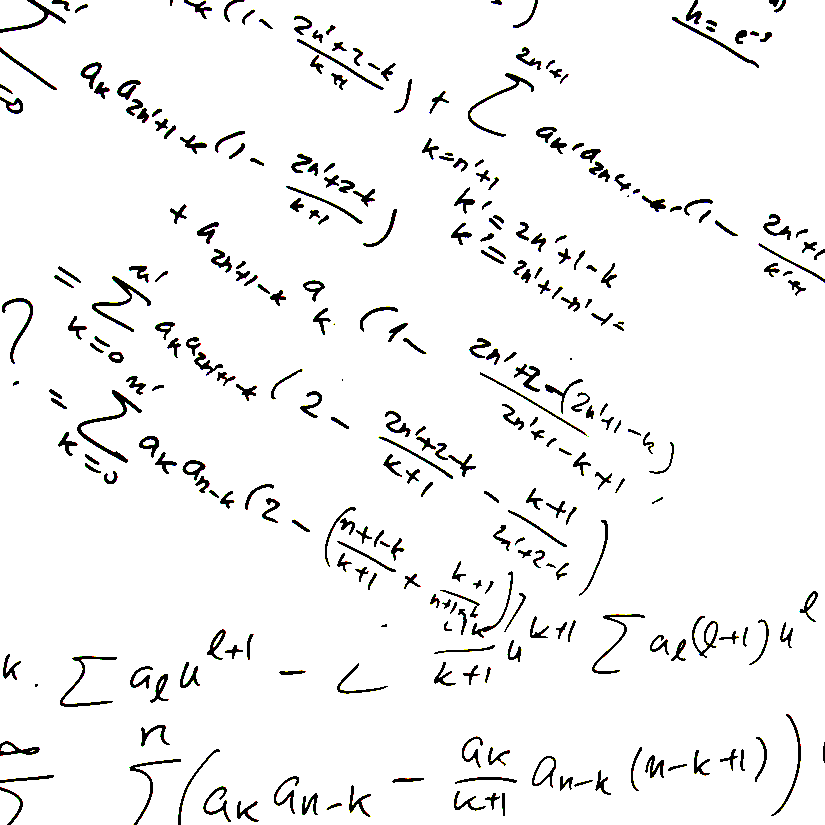
\includegraphics[width=8cm]{titlepic.png}
	};
\end{tikzpicture}
}

\usepackage[math]{iwona}

\newcommand{\hplus}{\mathbin{\hat+}}
\newcommand{\hdot}{\mathbin{\hat\cdot}}
% Описание теорем
\newtheorem{theorem}{Теорема}
\newtheorem{seq}{Следствие}
%%

\LECT % 

% Титульный лист теорем
\author[Д.\,В. Чупраков]{канд.\,физ.-матем.\,наук, доцент Д.\,В. Чупраков\\[6pt] usr10381@vyatsu.ru}

\institute[ВятГУ]{ФГБОУ ВО Вятский государственный университет}

\department{Факультет экономики и финансов}

\title[Лекция~17. Статистические оценки]{
	Введение в экономико-математическое моделирование\\[12pt]
	Лекция~16. Статистические оценки}
\date{9 декабря 2020~г.}


\setbeamercovered{invisible}

\setbeamercolor{math text}{fg=vgured!70!black}


\begin{document}


\maketitle

% \begin{frame}{Структура лекции}{}
% 	\tableofcontents
% \end{frame}

\section{Выборочный метод}

\begin{frame}{Статистическая оценка}
    Приближенное значение $\theta^*$ характеристики $\theta$ случайной величины $X$, вычисленное по выборке~$V$ называется \alert{статистической оценкой} характеристики $\theta$.

    \bigskip
    {\centering
    \begin{tikzpicture}[>=latex]
        \node[draw, fill=vgublue, text=white] (A) at (0,0) {Статистические оценки};
        \node[draw] (B) at (-3,-2) {Точечные};
        \node[draw] (C) at (3,-2) { Интервальные};
        \draw[->,thick] (A) edge (B) edge (C);
    \end{tikzpicture}
    \par}

    \bigskip
    \begin{block}{}
    \begin{itemize}
        \item Оценка определяемая одним числом, называется \alert{точечной}.
        \item Промежуток, который  с некоторой вероятностью накрывает значение характеристики $\theta$ называется \alert{интервальной} оценкой.
    \end{itemize}
    \end{block}
    
\end{frame}

\begin{frame}{Три орешка для Золушки}{}
    \begin{itemize}
        \item \alert{Несмещенность}~--- среднее значение оценок $\theta^*(V)$ по~всевозможным выборкам равно оцениваемой характеристике $\theta$:
            $$
                M \big(\theta^*(V) \big)= \theta
            $$
        
        \item \alert{Состоятельность}~--- с увеличением числа опытов $n$ случайная величина $\theta^*$ приближается к $\theta$
        $$
            |\theta^*(V_n) - \theta| \xrightarrow{n \to N} 0 
        $$
        \item \alert{Эффективность}~--- оценка $\theta^*$ обладает  наименьшей дисперсией по сравнению с другими оценками параметра $\theta$:
        $$
            D(\theta^*) \xrightarrow{\theta^*} \min
        $$
    \end{itemize}
\end{frame}
\begin{frame}{}{}
    Каждая несмещенная оценка характеризуется своей дисперсией.
\end{frame}

\begin{frame}{Генеральная доля}{}

    Пусть признаком~$A$ обладают $M$ элементов генеральной совокупности, содержащей $N$ элементов.
    \medskip

    
    Рассмотрим в качестве оценки выборочную долю $w =m/n$ элементов обладающих признаком~$А$ в выборке.

    \begin{theorem}    
        Выборочная доля $\omega = \frac{m}{n}$ является несмещенной и состоятельной оценкой генеральной доли $p = \frac{M}{N}$. 

        Дисперсия оценки равна $\sigma_w$
    \end{theorem}

    \bigskip
    {\centering
    \begin{tikzpicture}[>=latex,y=9mm]
        \node[draw, fill=vgublue, text=white] (A) at (0,0) {Выборка};
        \node[draw,ellipse] (B) at (-3,0) {Повторная};
        \node[draw,ellipse] (C) at (3.5,0) {Бесповторная};
        \node[draw] (BT) at (-3,-2) {$\sigma_w=\dfrac{pq}{n}$};
        \node[draw] (CT) at (3.5,-2) {$\sigma_w=\dfrac{pq}{n}\left(\dfrac{N-n}{N-1}\right)$};
        \draw[thick] (A) edge (B) edge (C);
        \draw[thick,->] (B) edge (BT);
        \draw[thick,->] (C) edge (CT);
    \end{tikzpicture}
    \par}

    \bigskip

\end{frame}

\begin{frame}{Генеральное среднее}{}

    \begin{theorem}    
        Выборочная средняя $\bar{x}_\text{в}$ есть несмещенная и состоятельная оценка генеральной совокупности $\bar{x}$.

        Дисперсия оценки равна $\sigma_{\bar{x}}$
    \end{theorem}

    \bigskip
    {\centering
    \begin{tikzpicture}[>=latex,y=9mm]
        \node[draw, fill=vgublue, text=white] (A) at (0,0) {Выборка};
        \node[draw,ellipse] (B) at (-3,0) {Повторная};
        \node[draw,ellipse] (C) at (3.5,0) {Бесповторная};
        \node[draw] (BT) at (-3,-2) {$\sigma_{\bar{x}}=\dfrac{\sigma^2}{n}$};
        \node[draw] (CT) at (3.5,-2) {$\sigma_{\bar{x}}=\dfrac{\sigma^2}{n}\left(\dfrac{N-n}{N-1}\right)$};
        \draw[thick] (A) edge (B) edge (C);
        \draw[thick,->] (B) edge (BT);
        \draw[thick,->] (C) edge (CT);
    \end{tikzpicture}
    \par}

    \bigskip
    \hrule
    \medskip
    При нормальном распределении величины $X$ среднее выборочное $\bar{x}_\text{в}$ будет эффективной оценкой генеральной средней
\end{frame}


\begin{frame}{Генеральная дисперсия}{}
    Генеральную дисперсию $\sigma^2$ оценим выборочной дисперсией $s^2$?
    
    \medskip
    \pause
    Это не лучший выбор:
    \begin{theorem}
        Выборочная дисперсия $s^2$ является \underline{смещенной}, но~состоятельная оценкой  генеральной дисперсии $\sigma^2$.
    \end{theorem}
    \pause
    Рассмотрим \alert{исправленную выборочную дисперсию}:
    $$
    \hat{s}^2 = \frac{n}{n-1}s^2
    $$
    \begin{theorem}
        Исправленная выборочная дисперсия $\hat{s}^2$ является \underline{несмещенной} и состоятельная оценкой  генеральной дисперсии $\sigma^2$.
    \end{theorem}
\end{frame}

\begin{frame}{Оценка закона распределения}{}
    \begin{theorem}
        Эмпирическая функция распределения выборки $F^*(x)$, построенная по статистическому дискретному ряду, является несмещенной состоятельной оценкой функции распределения $F(x)$ случайной величины $X$.
    \end{theorem}
\end{frame}
\begin{frame}{Проблема точечных оценок}{}
    Допустим, мы нашли способ по выборке~$V$ оценить неизвестный параметр~$\theta$.

    
    Точечная оценка зависит от элементов в выборке, поэтому она случайна.
    
    Использование точечной оценки может привести к существенным ошибкам.

    Как оценить надёжность замены реального параметра $\theta$ его точечной оценкой $\theta^*$? 

\end{frame}

% \begin{frame}{Интервальная оценка}{}

% \end{frame}

\begin{frame}{Доверительный интервал}{}
    Рассмотрим промежуток $[\theta^*-\varepsilon; \theta^*+\varepsilon]$
    
    \alert{Доверительная вероятность $\gamma$}~--- вероятность накрыть интервалом $[\theta^*-\varepsilon; \theta^*+\varepsilon]$ величину характеристики $\theta$:
    $$
        \gamma = P(\theta^*-\varepsilon \leqslant \theta \leqslant \theta^*+\varepsilon)
    $$

    \alert{Доверительный интервал:}
    $$
        I_\gamma = [\theta^*-\varepsilon; \theta^*+\varepsilon]
    $$
\end{frame}

\begin{frame}{Свойства интервальной оценки}{}
\begin{itemize}
    \item Параметр~$\varepsilon$~--- \alert{точность доверительного интервала}
    
    \smallskip
    \hfill Чем меньше $\varepsilon$, тем точнее интервальная оценка.

    \item Параметр~$\gamma$~--- \alert{надежность доверительного интервала}
    
    \smallskip
    \hfill Чем больше $\gamma$, тем надежнее интервал.
\end{itemize}

\vfill
\begin{alertblock}{Противоречивость параметров}
    При фиксированном размере выборки выборке увеличение точности ведет к снижению надежности и наоборот.
\end{alertblock}

\end{frame}

\begin{frame}{}{}
    \centering

    Доверительные интервалы\\ для параметров нормального распределения
   
\end{frame}
\begin{frame}[allowframebreaks]{Интервал для генеральной выборочной}{}
    $$
    X \sim N(\mu,\sigma)
    $$
    
    Найдем доверительный интервал для $\bar{x}$ с надежностью $\gamma$

    Выборка
    $$
    X_1, X_2, \ldots,~X_n
    $$
    \begin{itemize}
        \item С.\,В. $X_i$~--- независимы,
        \item $X_i\sim N(\mu,\sigma )$
    \end{itemize}
    
    Значит,
    \begin{gather*}
        M(X_1) = M(X_2) = \ldots = M(X_n) = M(X) = \mu, \\
        D(X_1) = D(X_2) = \ldots  = D(X_n) = D(X) = \sigma^2.
    \end{gather*}
    
    \framebreak
    
    Выборочное среднее  $\overline{X}_\text{в}$  также будет распределено по нормальному закону.
    
    Найдем параметры распределения:

    \structure{Математическое ожидание:}

      
    \begin{multline*}
        M(\overline{X}_\text{в}) 
        = M \left(\frac{1}{n}\sum_{i=1}^n X_i \right) 
        = \frac{1}{n}\sum_{i=1}^n M(X_i)
        = \frac{1}{n}\sum_{i=1}^n M(X)
        =\\
        = \frac{1}{n}\cdot n\cdot M(X) 
        =  M(X)
        = \bar{x}
    \end{multline*}
    \framebreak
  
    \structure{Дисперсия:}

    \begin{multline*}
        D(\overline{X}_\text{в})
        = D \left(\frac{1}{n}\sum_{i=1}^n X_i \right) 
        = \frac{1}{n^2}\sum_{i=1}^n D(X_i)
        = \frac{1}{n^2}\sum_{i=1}^n D(X)
        =\\
        = \frac{1}{n^2}\cdot n\cdot D(X) 
        =  \frac{D(X)}{n}
        =  \frac{\sigma^2}{n}
        = \sigma_{\bar{x}}^2
    \end{multline*}

    Итак,   
    $$ 
        M(\overline{X}_\text{в} )= \bar{x} \qquad   D(\overline{X}_\text{в})=\sigma_{\bar x}^2
    $$
    \framebreak

     Воспользуемся формулой вероятности отклонения С.В. $X\sim N(\mu,\sigma)$ от своего математического ожидания на величину, не превосходящую $\Delta$:
    %  $$
    %      P(|X-\mu|< \Delta) = 2\Phi\left(\frac{\Delta}l{\sigma }\right)
    %  $$ 


    $$
       \gamma = P(|\bar{x}_\text{в} - \bar{x}| < \Delta) = 2\Phi \left(\frac{\Delta }{\sigma_{\bar x}}\right) = 2\Phi(t),
    $$
    $$
       t=\frac{\Delta}{\sigma_{\bar x}},\quad \sigma_{\bar x}=\sqrt{\frac{D(X)} n}
    $$

% Откуда  $\Delta =t\cdot \sigma _{\bar x}$  поэтому 

% \begin{equation*}
% \gamma =P(|\bar x-\bar x_{\Gamma }|<t\cdot \sigma _{\bar x})=2\Phi \left(t\right)
% \end{equation*}

\framebreak
\begin{theorem}
    Доверительный интервал для  $\bar x$  
 есть  
 $$
    \left(\bar x-t\cdot \sigma _{\bar x};\bar x+t\cdot \sigma_{\bar x}\right)
 $$  
 где~$t$ определяется из уравнения $\Phi (t)= \gamma/2$. 
\end{theorem}

\bigskip
{\centering
\begin{tikzpicture}[>=latex,y=9mm]
    \node[draw, fill=vgublue, text=white] (A) at (0,0) {Выборка};
    \node[draw,ellipse] (B) at (-3,0) {Повторная};
    \node[draw,ellipse] (C) at (3.5,0) {Бесповторная};
    \node[draw] (BT) at (-3,-2) {$\sigma_{\bar{x}}=\dfrac{\sigma^2}{n}\approx \dfrac{s^2}{n}$};
    \node[draw] (CT) at (3.5,-2) {$\sigma_{\bar{x}}=\dfrac{\sigma^2}{n}\left(\dfrac{N-n}{N-1}\right)\approx \dfrac{s^2}{n}\left(1-\dfrac{n}{N}\right)$};
    \draw[thick] (A) edge (B) edge (C);
    \draw[thick,->] (B) edge (BT);
    \draw[thick,->] (C) edge (CT);
\end{tikzpicture}
\par}

\end{frame}

\begin{frame}{Интервальные оценки}{}
    \begin{tabular}{lcc}
        \hline
        Параметр         & Генеральная средняя  & Генеральная доля \\
        \hline
        Интервал &$|\bar{x} - \bar{x}_\text{в}| \leqslant \Delta$ & $|p - \omega_\text{в}| \leqslant \Delta$\\
        &  $ \bar{x}_\text{в} - \Delta \leqslant \bar{x} \leqslant \bar{x}_\text{в} + \Delta$ & $ w - \Delta \leqslant p \leqslant w + \Delta$\\[8pt]
        Отклонение & $\Delta = t\sigma_{\overline{x}}$ & $\Delta = t\sigma_\omega$\\
         & $ \gamma = 2\Phi(t)$ & $\gamma = 2\Phi(t)$ \\[13pt]
        % \hline
        \multicolumn{3}{l}{\structure{Тип выборки}}\\[8pt]
        % \hline
        Повторная 
            & $\sigma_x = \sqrt{\frac{\sigma^2}{n}}$ 
            & $\sigma_w  = \sqrt{\frac{p(1-p)}{n}}$
        \\
            & $\sigma_x \approx \sqrt{\frac{s^2}{n}}$ 
            & $\sigma_w  \approx \sqrt{\frac{\omega(1-\omega)}{n}}$
        \\[8pt]
        Бесповторная  
            & $\sigma_x = \sqrt{\frac{\sigma^2}{n}\left(\frac{N-n}{N-1}\right)}$
            & $\sigma_w = \sqrt{\frac{p(1-p)}{n}\left(\frac{N-n}{N-1}\right)}$
        \\
            & $\sigma_x \approx \sqrt{\frac{s^2}{n}\left(1-\frac{n}{N}\right)}$
            & $\sigma_w  \approx \sqrt{\frac{\omega(1-\omega)}{n}\left(1-\frac{n}{N}\right)}$
        \\
        \hline
        % Параметр~$t$ & \multicolumn{2}{c}{$\gamma = 2\Phi(t)$} \\
        % Объем повторной выборки & $n=\frac{t^2\sigma}{\Delta}$ & $n=\frac{t^2pq}{\Delta}$\\ 
        % Объем бесповторной  выборки & \multicolumn{2}{c}{$n'=\frac{nN}{n+N}$}\\ 
        % \hline
    \end{tabular}
\end{frame}


\begin{frame}[allowframebreaks]{Пример}
    \begin{exampleblock}{}
        Случайная величина~$X$ имеет нормальное распределение с известным средним квадратическим отклонением $\sigma=3$. 

        Найти доверительный интервал для оценки неизвестного математического ожидания $\mu$ по выборочным средним $\bar{x}$, если объем выборки $n = 36$ и задана надежность оценки $\gamma= 0.95$.
    \end{exampleblock}
    \begin{itemize}
        \item Так как объем генеральной совокупности не указан, считаем выборку повтороной.
        \item Найдем параметр $t$. 
        \begin{gather*}
            2\Phi(t) = 0.95\\
            \Phi(t) = 0.475\\
            t \approx 1.96
        \end{gather*}
        \item Найдем $\sigma_{\bar{x}}$:
        $$
            \sigma_{\bar{x}} = \sqrt{\frac{\sigma^2}{n}} 
            = \sqrt{\frac{3^2}{36}} 
            = \frac{1}{2}. 
        $$
        \item Найдем точность 
        $$
            \Delta = t\sigma_{\bar{x}} = \frac{1.96}{2}=0.98
        $$
    \end{itemize}
    \structure{Ответ:} Математическое ожидание отклоняется от выборочного математического ожидания не более чем на 0.98.
\end{frame}


\begin{frame}{Пример}
    \begin{exampleblock}{}
        С целью размещения рекламы опрошено 420 телезрителей, из которых данную передачу смотрят 170 человек. 
        С доверительной вероятностью $\gamma=0.91$ найти долю телезрителей, охваченных рекламой в лучшем случае.        
    \end{exampleblock}
    \begin{itemize}
        \item Объем генеральной совокупности не известен. Считаем выборку посторной.
        \item Для оценки неизвестной доли телезрителей используем  доверительный интервал:
        $$ 
            w - \Delta \leqslant p \leqslant w + \Delta,\qquad \Delta = t\sigma_{\bar{x}}, \quad \gamma=2\Phi(t)
        $$
        \item Найдем выборочную долю: 
        $$
            w= \frac{170}{420} \approx 0.405
        $$
        \item Найдем параметр $t$. 
        \begin{gather*}
            2\Phi(t) = 0.91\\
            \Phi(t) = 0.455\\
            t \approx 1.70
        \end{gather*}    
        \item Найдем $\sigma_{\bar{x}}\approx \sqrt{\frac{w(1-w)}{n}} = \sqrt{\frac{0.405\cdot(1-0,405)}{420}}\approx 0,0240 $
        
        \item Найдем точность
        $$
            \Delta = 1.70\cdot 0.00074=0.0013
        $$
        $$ 
            0.405 - 0.0240 \leqslant p \leqslant 0.455 - 0.0240 
        $$
        $$ 
            0.381 \leqslant p \leqslant 0.429
        $$
    \end{itemize}
        Ответ: В лучшем случае рекламой охвачено $42.9\%$ телезрителей.
\end{frame}


\begin{frame}{Оценка объема выборки}
    Объем выборки влияет на качество выборочного исследования и определяет необходимые временные, трудовые и стоимостные затраты.

    \begin{block}{}
    Для определения объема выборки $n$ необходимо задать два параметра:
    \begin{itemize}
        \item надежность $\gamma$ оценки исследуемой характеристики
        \item точность $\Delta$ оценки исследуемой характеристики
    \end{itemize}
    \end{block}
    

\end{frame}
\begin{frame}{Объем выборки}
    
    \structure{Объем повторной  выборки}
    
    \bigskip
    {\centering
\begin{tikzpicture}[>=latex,y=9mm]
    \node[draw, fill=vgublue, text=white,ellipse] (A) at (0,0) {Характеристика};
    \node[draw,ellipse] (B) at (-2,-1.5) {Среднее};
    \node[draw,ellipse] (C) at (2,-1.5) {Доля};
    \node[draw] (BT) at (-4,-3) {$n=\dfrac{t^2\sigma^2}{\Delta^2}$};
    \node[draw] (CT) at (4,-3) {$n=\dfrac{t^2pq}{\Delta^2}$};
    \draw[thick] (A) edge (B) edge (C);
    \draw[thick,->] (B) edge (BT);
    \draw[thick,->] (C) edge (CT);
\end{tikzpicture}
\par}

\bigskip

\structure{Объем бесповторной  выборки}

$$
    n'=\frac{nN}{n+N}
$$ 
% \textit{Объем бесповторной  выборки всегда меньше объема соответсвующей повторной выборки.}
\end{frame}

\begin{frame}[allowframebreaks]{Пример вычисления объема выборки}
    \begin{exampleblock}{}
        Строительная компания хочет оценить среднюю стоимость ремонтных работ, выполняемых для клиентов. 
        Каким должен быть объем бесповторной выборки среди 1200 клиентов строительной фирмы, если среднее квадратическое отклонение по результатам пробного обследования составило 85 тыс.~руб., а предельная ошибка выборки не должна превышать 20 тыс.~руб с вероятностью 0.95?
    \end{exampleblock}
    \begin{itemize}
        \item Имеем $N=1200$, $\gamma=0.95$, $\Delta= 20$, $\sigma=85$
        \item Найдем параметр $t$
        \begin{gather*}
            2\Phi(t) = 0.95\\
            \Phi(t) = 0.475\\
            t \approx 1.96
        \end{gather*}
        \item Найдем объем повторной выборки для оценки средней стоимости: 
        $$
            n=\frac{t^2\sigma^2}{\Delta^2} = \frac{1.96^2 \cdot 85^2}{20^2} \approx 69.3889
        $$
        Не округляем, так как это промежуточный результат.
        \item Найдем объем бесповторной выборки 
        $$
            n'= \frac{nN}{n+N}= \frac{69.3889 \cdot 1200}{69.3889+1200}\approx 66
        $$
        Округляем в большую сторону.
    \end{itemize}
    \structure{Ответ:} Достаточно исследовать данные работ по 66 клиентам.

\end{frame}

\begin{frame}[t]{Квантиль}{}
    \begin{block}{}
        \alert{$\alpha$-квант\'{и}ль} распределения~--- такое значение $x_\alpha$, что для С.\,В. $X$, имеющей данное распределение,  выполнено свойство  
        $$
            P(X< x_\alpha) = \alpha
        $$
    \end{block}
    
    \vfill
    \alert{$p$-й Перцентиль}~---  квантиль уровня $\alpha= \frac{p}{100}$
\end{frame}
\begin{frame}[allowframebreaks]{Оценка дисперсии}
Найдем доверительный интервал для среднего квадратического отклонения нормально распределенной величины
$$
    X\sim N(\bar{x},\sigma)
$$
с заданной надежностью $\gamma$



Если  \structure{генеральное среднее $\bar x$  известно}, то доверительный интервал для генеральной дисперсии $\sigma^2$
имеет вид:  
$$
    \frac{ns^2}{\chi _2^2} < \sigma < \frac{ns^2}{\chi _1^2},
$$ 
где 
\begin{itemize}
    \item $n$~--- объем выборки
    \item $\chi _1^2=\chi_{\frac{1+\gamma } 2,n}^2$ , $\chi _2^2=\chi_{\frac{1-\gamma } 2,n}^2$~--- квантили  $\chi^2$\nobreakdash-распределения с $n$ степенями свободы.
\end{itemize}

\framebreak

 Если \structure{математическое ожидание  $\bar x$  неизвестно}, то доверительный интервал для генеральной дисперсии $\sigma^2$ имеет вид: 
    $$
      \frac{(n-1)\hat{s}^2}{\chi_2^2} < \sigma < \frac{(n-1)\hat{s}^2}{\chi_1^2},
    $$
    где 
\begin{itemize}
    \item $n$~--- объем выборки
    \item $\chi _1^2=\chi_{\frac{1+\gamma } 2,n-1}^2$ , $\chi _2^2=\chi_{\frac{1-\gamma } 2,n-1}^2$~--- квантили  $\chi ^2$\nobreakdash-распределения с $n-1$ степенями свободы.
\end{itemize}
\end{frame}


\begin{frame}[allowframebreaks]{Пример оценки дисперсии}{}
    \begin{exampleblock}{}
        Для оценки параметра нормально распределенной случайной величины была сделана выборка объема в 30 единиц и вычислено $s = 1.5$.
        Найти доверительный интервал, покрывающий $\sigma$ с надежностью $\gamma =  0.90$.
    \end{exampleblock}
    \begin{itemize}
    \item Имеем $n = 30$, $\gamma = 0.9$.
    \item Математическое ожидание не известно.
    \item Исправим дисперсию $\hat{s}^2 = \frac{30}{29} (1.5)^2 \approx 2.328$
    \item Вычислим квантили 
         \begin{align*}
             \chi^2_1 &= \chi^2_{\frac{1+0.9}{2},30-1} = \chi^2_{0.95, 29} =17.7\\
             \chi^2_2 &= \chi^2_{\frac{1-0.9}{2},30-1} = \chi^2_{0.05,29} = 42.6
         \end{align*}
     \item Найдем интервал
     \begin{gather*}
        \frac{n-1}{\chi^2_2}\hat{s}^2 < \sigma^2 < \frac{\sqrt{n-1} \hat{s}^2}{\chi^2_1}\\
         \frac{29 \cdot  2.328}{42.6} < \sigma < \frac{ 29 \cdot 2.328}{17.76}\\
         1,585 < \sigma^217 < 1.579 
     \end{gather*}
    \end{itemize}
\end{frame}

\end{document}



При обработке статистической информации широко используют распределение статистик, которые вычисляются по выборке из нормально распределенной генеральной совокупности.
Квантилью порядка р распределения случайной величины X называется действительное число, удовлетворяющее уравнению P(X<. (определяются по специальным стат.таблицам)

\section{Интервальные оценки}
\begin{frame}[t]{}{}
\vspace{2cm}
{\LARGE	Интервальные оценка\par}
\vspace{\fill}

\subsection{Интервальная оценка}

\begin{frame}{Интервальнаяая оценка}{}
\begin{tabular}{m{0.65\textwidth}m{0.33\textwidth}}
\structure{Определение}

 $\Phi$ \alert{Интервальная оценка} - числовой интервал, определяемый двумя числами, содержащий неизвестный параметр генеральной совокупности. 
 
 \\Интервальная оценка более информативная, чем точечная оценка.  
 
 \\Если для произвольного числа \epsilon >0 выполняется неравенство |\theta  - \theta ^*|<\epsilon, то положительное число \epsilon характеризует точность оценки. В интервальной оценке устанавливается $\Phi$ \alert{доверительная вероятность \left(надежность \right), с которой эта оценка накроет неизвестный параметр, то есть это вероятность p, с которой выполяется неравенство |\theta  - \theta ^*|<\epsilon.
 
 \\Часто надежность принимают равной 0,9; 0,95; 0,99; 0,999.

\end{tabular}

\end{frame}

\subsection{Доверительный интервал}
\begin{frame}{Доверительный интервал}{}
\begin{tabular}{m{0.65\textwidth}m{0.33\textwidth}}
\structure{Определение}

 $\Phi$ \alert{Доверительным интервалом} называют найденный по данным выборки интервал \left (\theta^*  - \epsilon; \theta ^* + \epsilon \right) , длина которого равна 2\epsilon и является функцией результатов наблюдений.

\end{tabular}

\end{frame}


\subsection{Доверительный интервал}
\begin{frame}{Доверительный интервал для математического ожидания}{}
\begin{tabular}{m{0.65\textwidth}m{0.33\textwidth}}


 \\Доверительный интервал для математического ожидания при известном \sigma. В некоторых случаях квадратическое отклонение ошибки измерения, а вместе с нею т самого измерения бывает известно.
 
\\ Доверительный интервал для математического ожидания при неизвестном \sigma. Пусть случайная величина X имеет нормальное распределение с известными нам параметрами \mu и \sigma , и не зависящее от них. В этом случае используетсы распределение Стьюдента и интервальной оценкой математического ожидания генеральной совокупности с заданной надежностью p будет являться интервал 

$ \left(x - t_p\left(f\right)*\frac s \sqrt n ; x+t_p\left(f\right)*\frac s \sqrt n \right)$
\\с границей доверительного интервала \left(точность оценки \right) \epsilon = t_p\left(f\right)*\frac s \sqrt n .
\end{tabular}

\end{frame}


\subsection{Доверительный интервал}
\begin{frame}{Доверительный интервал для среднего квадратического отклонения}{}
\begin{tabular}{m{0.65\textwidth}m{0.33\textwidth}}


 \\Доверительный интервал для среднего квадратического отклонения \sigma. С надежностью p можно утверждать, что доверительный интервал \left(s - sq; s + sq \right) покрывает неизвестный параметр с точностью оценки \epsilon =sq . 

\end{tabular}

\end{frame}

\subsection{Примеры решения задач}
\begin{frame}{Примеры решения задач}{}
\begin{tabular}{m{0.65\textwidth}m{0.33\textwidth}}

$\Phi$ \alert{Пример 1:}
\\Случайная величина X имеет нормальное распределение с известным средним квадратическим отклонением \sigma =3. Найти доверительные интервалы для оценки неизвестноо математического ожидания \alpha по выборочным средним x, если объем выборки n = 36 и задана надежность оценки p= 0,95.
 
$\Phi$ \alert{Решение}
\\Найдем t. Из соотношения 2Ф\left (t \right) = 0,95 получим Ф\left( t \right) = 0,475. По таблице значений интегральной функции Лапласа находим t = 1,96. Найдем точность оценки \delta = \frac t*\sigma \sqrt n = \left(1,96*3 \right)/\sqrt 36 = 0,98. Доверительный интервал следующий: \left(x - 0,98; x + 0,98 \right). 

\end{tabular}
\end{frame}


\begin{frame}{Примеры решения задач}{}
\begin{tabular}{m{0.65\textwidth}m{0.33\textwidth}}

$\Phi$ \alert{Пример 2:}
\\При доверительной вероятности 90\%  найти доверительный интервал для D(x), если для выборки, объемом 5 выборочная D(x) = 6,6, а выборочная средняя 0,4.
 
$\Phi$ \alert{Решение}
\\По таблицам распределения \chi^2 найдем значение критерия \chi^2 для уровня значимости \upsilon =4 и \alpha =/2=0,05
\\ \chi^2_0,05;4=9,5
\\        \chi^2_\frac \alpha 2; \upsilon = \chi^2_0,95;4 = 0,711
\\ \frac 4*6,6 9,5 < \sigma^2 < \frac 4*6,6 0,711
2,78 < \sigma^2 < 37.13

\end{tabular}
\end{frame}


\begin{frame}{Примеры решения задач}{}
\begin{tabular}{m{0.65\textwidth}m{0.33\textwidth}}

$\Phi$ \alert{Пример 3:}
\\Признак X распределен в генеральной совокупности нормально. Найти доверительный интервал для \sigma с надежностью p=0,95 , если n=20, s=0,40.
 
$\Phi$ \alert{Решение}
\\Для надежности p=0,95 и n=20 найдем в таблице значений q=q\left( \gamma , n \right)  q=0,37. Далее s*q=0,40*0,37=0,148. Доверительный инетервал \left (0,40-0,15; 0,40+0,15 \right) , то есть \left( 0,25; 0,55 \right) покрывает \sigma с надежностью 0,95.

\end{tabular}
\end{frame}



\begin{frame}{Резюме}
	К настоящему моменту вы знаете:
	\begin{enumerate}
	\item 
		Точечную оценку 
	\item 
		Интервальную оценку
	\end{enumerate}
\end{frame}

\begin{frame}{Источники информации}
\begin{itemize}
\item 
	Статистические оценки параметров генеральной совокупности:  {\color{blue}\href{https://cloud.mail.ru/public/4SN3/2MJYgEz95}{Шилова З.\,В. , Шилов О.\,И.  Теория вероятностей и математическая статистика}} раздел 2 глава 2 с. 72--79, с. 88--90.
\end{itemize}

\end{frame}